\documentclass[11pt,italian]{article}
\usepackage[T1]{fontenc}
\usepackage[utf8]{inputenc} %utf8 % lettere accentate da tastiera
\usepackage[italian]{babel} % lingua del documento
\usepackage{blindtext}
\usepackage{enumitem}
\usepackage{graphicx}
\usepackage{float}
\usepackage{xcolor}   % for \textcolor
\usepackage[font=small,labelfont=bf,skip=10pt]{caption}
\setlength{\belowcaptionskip}{-10pt}
\usepackage{listings}
\lstset{
    basicstyle=\small\ttfamily,
    columns=fullflexible,
    frame=single,
    breaklines=true,
    postbreak=\mbox{\textcolor{red}{$\hookrightarrow$}\space},
    tabsize=4, % tab space width
    showstringspaces=false, % don't mark spaces in strings
    numbers=left, % display line numbers on the left
    commentstyle=\color[HTML]{a0a1a7}, % comment color
    keywordstyle=\color[HTML]{40a3f5}, % keyword color
    stringstyle=\color{red}, % string color,
    emphstyle={\color[HTML]{40a3f5}}
}
\usepackage{hyperref}
\usepackage{cleveref}
\hypersetup{
    colorlinks = true,
    linkbordercolor = {white},
    urlcolor = blue
}
\usepackage{graphicx}
\graphicspath{ {./images/} }

% Italian syntax spacing
\frenchspacing

% Line height
\renewcommand{\baselinestretch}{1.15}

% Use lstinline as item in description
\makeatletter
\newcommand*{\lstitem}[1][]{%
  \setbox0\hbox\bgroup
    \patchcmd{\lst@InlineM}{\@empty}{\@empty\egroup\item[\usebox0]\leavevmode\ignorespaces}{}{}%
    \lstinline[#1]%
}
\makeatother

\title{
    Metodi del Calcoli Scientifico \\
    \normalsize Compressione di immagini tramite DCT \\
    \normalsize Progetto 2 / Parte 2
}

\date{A.A.: 2019/2020}

\author{
    \normalsize
    \textsc{Edoardo Silva 816560} \\
    \normalsize
    \textsc{Bryan Zhigui 816335} \\
    \normalsize
    \textsc{Davide Marchetti 815990}
}

\begin{document}
\maketitle

\section{Abstract}
Si vuole presentare un software che implementa una compressione delle immagini basata sulla DCT.

Il programma deve permettere all’utente di scegliere da filesystem un'immagine bitmap in toni di grigio, applicarne la compressione secondo i parametri specificati e visualizzarne l'output.

\newpage
\section{Implementazione}
L'applicazione è scritta in Python utilizzando PyQT5 che agisce da wrapper per QtGUI: un framework per la scrittura di interfacce grafiche in C++.

Inoltre, PyQT5 è multipiattaforma e tramite Python è possibile creare applicazioni molto rapidamente senza perdere i benefici della velocità del C++.
I moduli utilizzati dalla nostra applicazione sono:
\begin{description}
    \lstitem{QtCore:} definisce una serie di classi utilizzabili per definire stili e comportamenti dei widget.
    \lstitem{QtGUI:} contiene utility per l'elaborazione di dati che interagiscono con componenti dei widget.
    \lstitem{QtWidgets:} racchiude tutta una collezione di widget grafici come pulsanti, label, slider, controlli per form e molto altro.
\end{description}
L'interfaccia grafica è disegnata con l'ausilio di \textbf{QtDesigner}, uno strumento facente parte del framework stesso.

Questo permette di ridurre notevolmente la complessità della creazione di un'applicazione, in quanto è necessario solamente implementare i metodi di gestione degli eventi e connetterli ai rispettivi componenti.

\newpage
\section{Interfaccia dell'applicazione}
In \cref{fig:application-window} riporta l’interfaccia dell'applicazione proposta all'utente e dotata delle seguenti caratteristiche:
\begin{itemize}
    \item Un pannello diviso in due sezioni per permettere di visualizzare affiancate: l’immagine originale e la rispettiva versione compressa.
    \item Un'area per scegliere un immagine da utilizzare come input con una checkbox per visualizzare l'immagine adattandola all'area predisposta.
    \item Una sezione nella quale regolare i parametri di compressione:
    \begin{enumerate}
        \item \textbf{$F$:} definisce la dimensione del blocco. L'immagine sarà suddivisa in blocchi $F\times F$ durante il processo di compressione.
        \item \textbf{$d$:} soglia di taglio delle frequenze di ogni blocco.
    \end{enumerate}
\end{itemize}

\begin{figure}[H]
    \makebox[\textwidth][c]{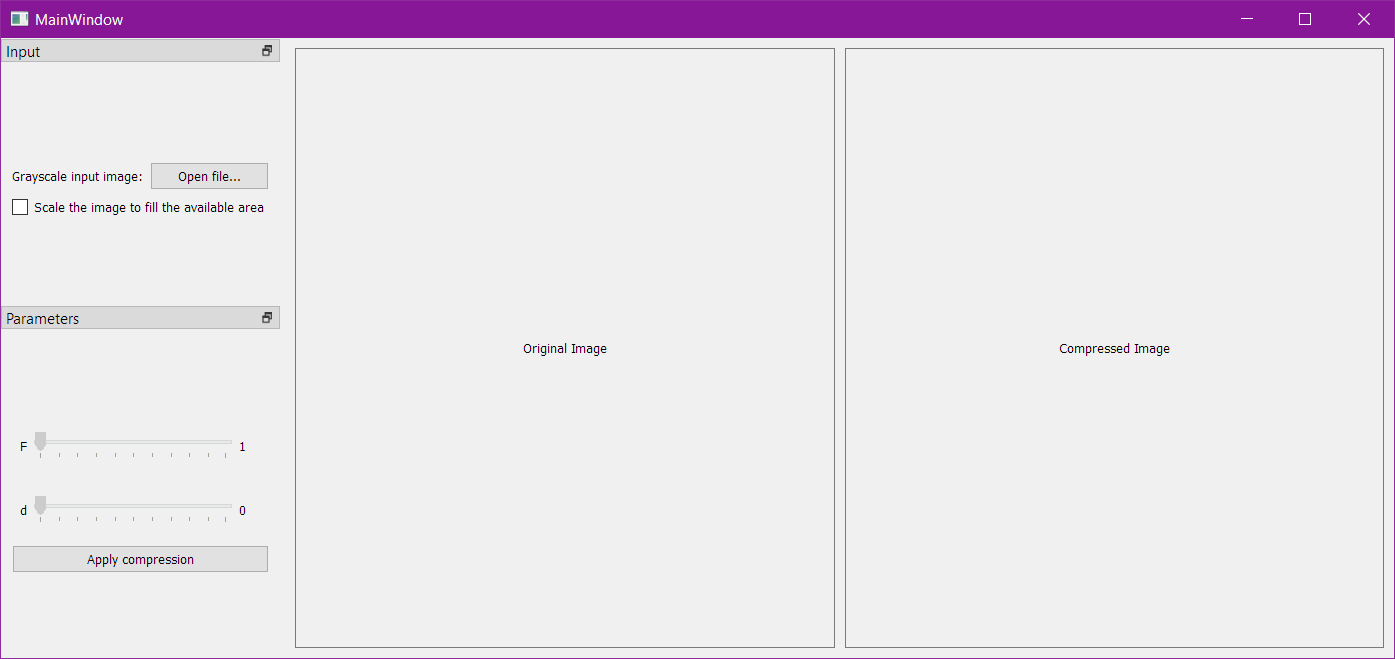
\includegraphics[width=1.4\linewidth]{application-window.png}}
    \caption{GUI dell'applicazione}
    \label{fig:application-window}
\end{figure}

\subsubsection*{Event handling}
Il listato \cref{code:event-handling} riporta la definizione del collegamento degli eventi dei widget dell'interfaccia al relativo gestore.
\begin{lstlisting}[language=Python,emph={self},label=code:event-handling,caption=Event-handling dei segnali dei widget]
def connectSignals(self):
    self.openFile.clicked.connect(self.ask_image)

    self.scaleImage.stateChanged.connect(self.updateImageScaling)

    self.fSlider.valueChanged.connect(self.updateFLabel)
    self.fSlider.valueChanged.connect(self.updateMaxDValue)

    self.dSlider.valueChanged.connect(self.updateDLabel)

    self.applyButton.clicked.connect(self.compress_image)

def updateImageScaling(self):
    for target in [self.originalImage, self.compressedImage]:
        target.setShouldScale(self.scaleImage.isChecked())

def updateFLabel(self):
    self.fValue.setText(str(self.fSlider.value()))

def updateDLabel(self):
    self.dValue.setText(str(self.dSlider.value()))

def updateMaxDValue(self):
    if self.fSlider.value() == 1:
        self.dSlider.setValue(0)
        self.dSlider.setEnabled(False)
        return

    limit = 2*self.fSlider.value() - 2

    self.dSlider.setMaximum(limit)
    self.dSlider.setTickInterval(limit / 10)
    self.dSlider.setEnabled(True)
\end{lstlisting}

\newpage
\section{Funzionalità}
\subsection{Richiesta immagine}
Si richiede all’utente di selezione un'immagine \lstinline{.bmp} in scala di grigi. Attraverso il pulsante "open file" è possibile reperire delle immagini di esempio presenti nella cartella \lstinline{./resources}, oppure sceglierne una personalizzata dal proprio dispositivo.

La finestra di dialogo è predisposta per filtrare le immagini selezionabili imponendo la scelta di immagini con estensione \lstinline{.bmp}. All'apertura viene effettuato il controllo che l'immagine sia effettivamente in scala di grigi. In caso di fallimento, sarà visualizzata una message box per notificarne l'errore.

\begin{figure}[H]
    \makebox[\textwidth][c]{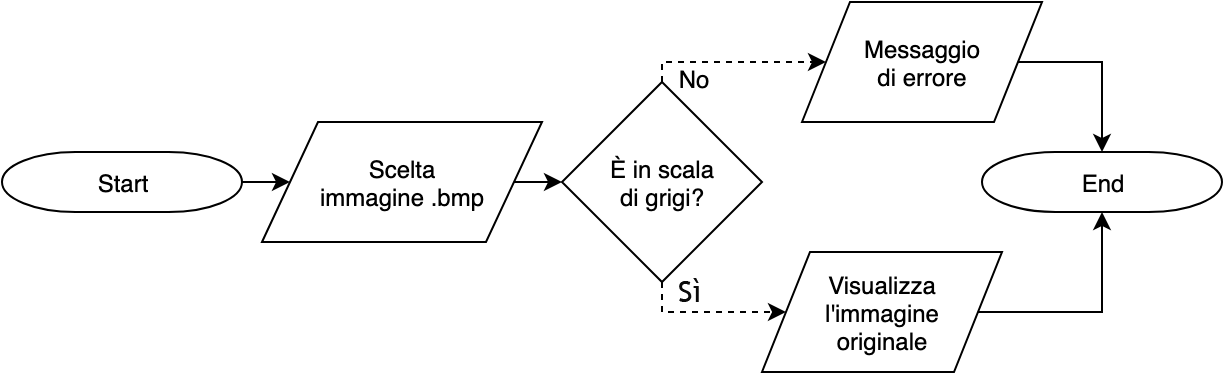
\includegraphics[width=1\linewidth]{flow-image-pick.png}}
    \caption{Flowchart di scelta dell'immagine}
    \label{fig:flow-image-pick}
\end{figure}

\noindent
L’immagine viene caricata nella prima sezione del pannello permettendo di scalarla come in \cref{fig:application-image-loaded}.
\begin{figure}[H]
    \makebox[\textwidth][c]{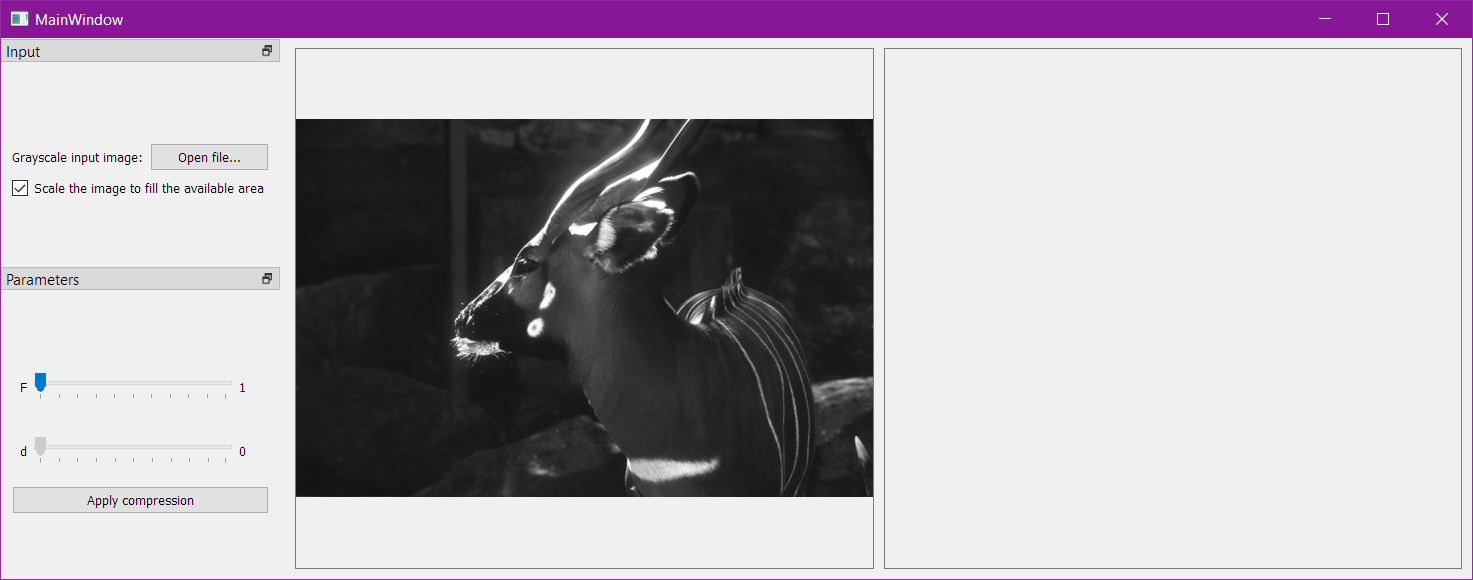
\includegraphics[width=1.15\linewidth]{application-image-loaded.png}}
    \caption{GUI: imagine caricata correttamente}
    \label{fig:application-image-loaded}
\end{figure}

\subsection{Compressione dell'immagine}
Per procedere con la compressione è necessario impostare i parametri $F$ e $d$. Questo permetterà di studiare gli effetti della compressione tramite alcuni esempi riportati nella \cref{section:examples}.

\subsubsection*{Note sulla compressione}
Solitamente, un’immagine a colori è composta da quattro canali ben distinti, identificati con la sigla \textbf{RGBA}: Red, Green, Blue e Alpha (Trasparency).
La loro combinazione permette la definizione di un qualunque colore.

La traccia richiede di lavorare con immagini in toni di grigio. Queste immagini verranno lette dall'applicazione come immagini a colori, tuttavia, questo non costituisce un problema.

La \cref{fig:channels} illustra come la rappresentazione di una determinata tonalità di grigio comporti lo stesso valore nelle componenti R, G e B.
\begin{figure}[H]
    \makebox[\textwidth][c]{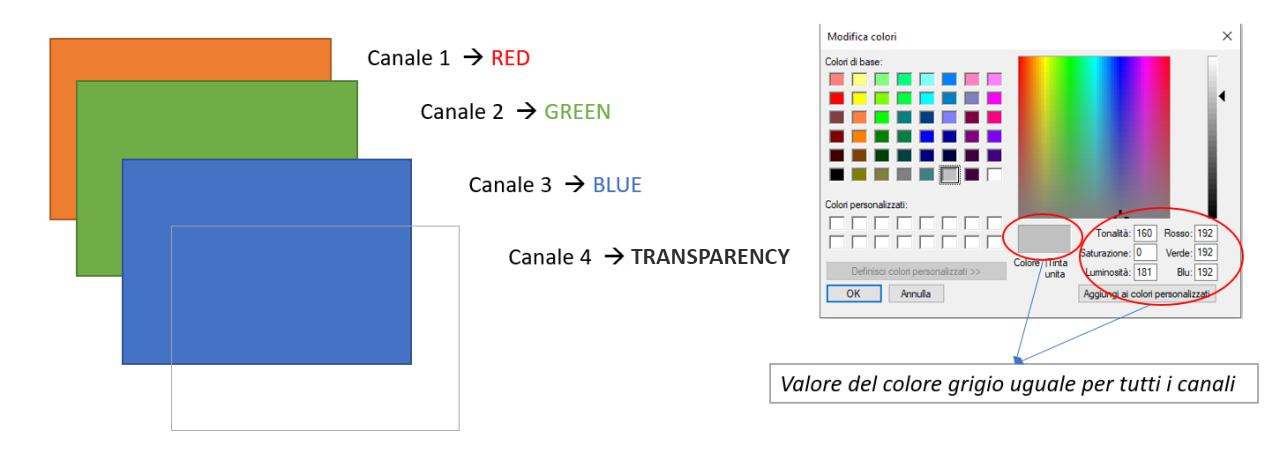
\includegraphics[width=1.2\linewidth]{channels.png}}
    \caption{Schema canali RGBA}
    \label{fig:channels}
\end{figure}

% Un’immagine viene rappresentata in termini di pixel e sappiamo che:
% \begin{itemize}
%     \item Un pixel equivale a 1Byte (ovvero 8 bit);
%     \item 1 Byte rappresenta un numero tra 0-255.
% \end{itemize}
\noindent
Il listato \ref{code:pixel-read} riporta le istruzioni di lettura ed estrazione dei pixel utilizzate dal nostro algoritmo.
Si può notare che dati i pixel di un immagine, si specifica il numero di byte presenti nella stessa ottenendo un buffer di dimensione \lstinline{altezza} $\times$ \lstinline{larghezza} $\times$ \lstinline{canali}.

Il buffer di bit viene suddiviso in gruppi da 8bit (\lstinline{uint8}) per ottenere i singoli byte di ciascuna componente dell'immagine. In conclusione, si estrae solamente il primo livello, che equivale alla componente \lstinline{R} dell'immagine.

I valori del singolo canale pur essendo interi vengono convertiti in float, per evitare troncamenti o overflow nell'applicazione della DCT negli step successivi.

\begin{lstlisting}[language=Python,label=code:pixel-read,caption=Estrazione del canale R dall'immagine]
# Source rappresenta la mappa dei pixel dell'immagine
values = source.constBits()
values.setsize(height * width * 4)

pixels = np.frombuffer(values, np.uint8).reshape((height, width, 4)).copy()
pixels = pixels[:, :, 0].astype(np.float)
\end{lstlisting}

\subsubsection*{Algoritmo}
\begin{figure}[H]
    \makebox[\textwidth][c]{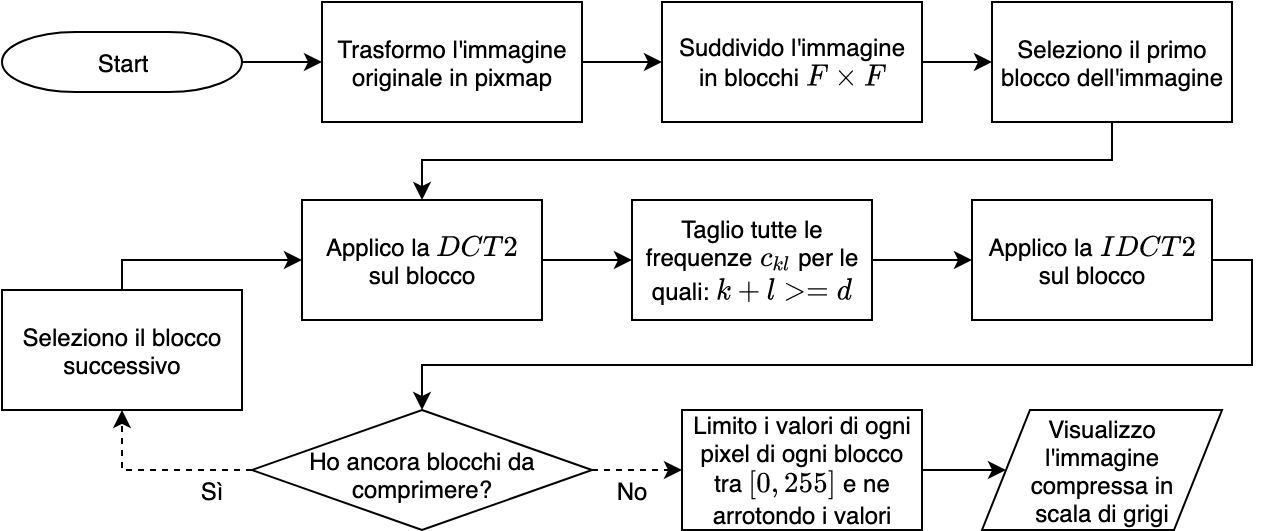
\includegraphics[width=1\linewidth]{flow-compression.png}}
    \caption{Flowchart di compressione dell'immagine}
    \label{fig:flow-compression}
\end{figure}

L'algoritmo implementato e riportato in \cref{fig:flow-compression} e nel listato \ref{code:algo-compression} lavora nel seguente modo:
\begin{enumerate}
    \item L’immagine originale viene trasformata in \lstinline{PixMap} dalla quale viene estratto uno tra i canali \lstinline{R}, \lstinline{G} e \lstinline{B}
	\item Vengono recuperati i valori di $F$ e $d$ immessi dall’utente
	\begin{enumerate}
		\item $F$ definisce l’ampiezza dei macro-blocchi
		\item $d$ regola da quale frequenza tagliare il blocco in fase di compressione
	\end{enumerate}
    \item L’immagine viene divisa in blocchi $z$ di dimensione $F\times F$ contenenti i rispettivi pixel dell'immagine originale, partendo dal primo blocco in alto a sinistra (\cref{fig:flow-compression-block}).

    \textbf{Nota:} Eventuali pixel per i quali non è possibile costruire un quadrato che li contenga, non verrranno compressi, e saranno una copia esatta dell'immagine originale.

	\item Per ogni blocco si effettuano le seguenti operazioni effettuando una sostituzione diretta nella matrice di pixel:
	\begin{enumerate}
		\item Si applica la $\mathit{DCT2}$ della libreria: $C = \mathit{DCT2}(z)$
		\item Vengono azzerate le frequenze $C_{kl}$ dove $k+l >= d$
		\item Si applica $\mathit{IDCT2}$ sulla matrice $C$: $z = \mathit{IDCT2}(C)$
	\end{enumerate}
	\item I valori della matrice di pixel vengono limitati tra $[0,255]$ e arrotondati all'intero più vicino
	\item La \lstinline{PixMap} viene riconvertita in immagine e visualizzata nella sezione dedicata
\end{enumerate}

\begin{figure}[H]
    \makebox[\textwidth][c]{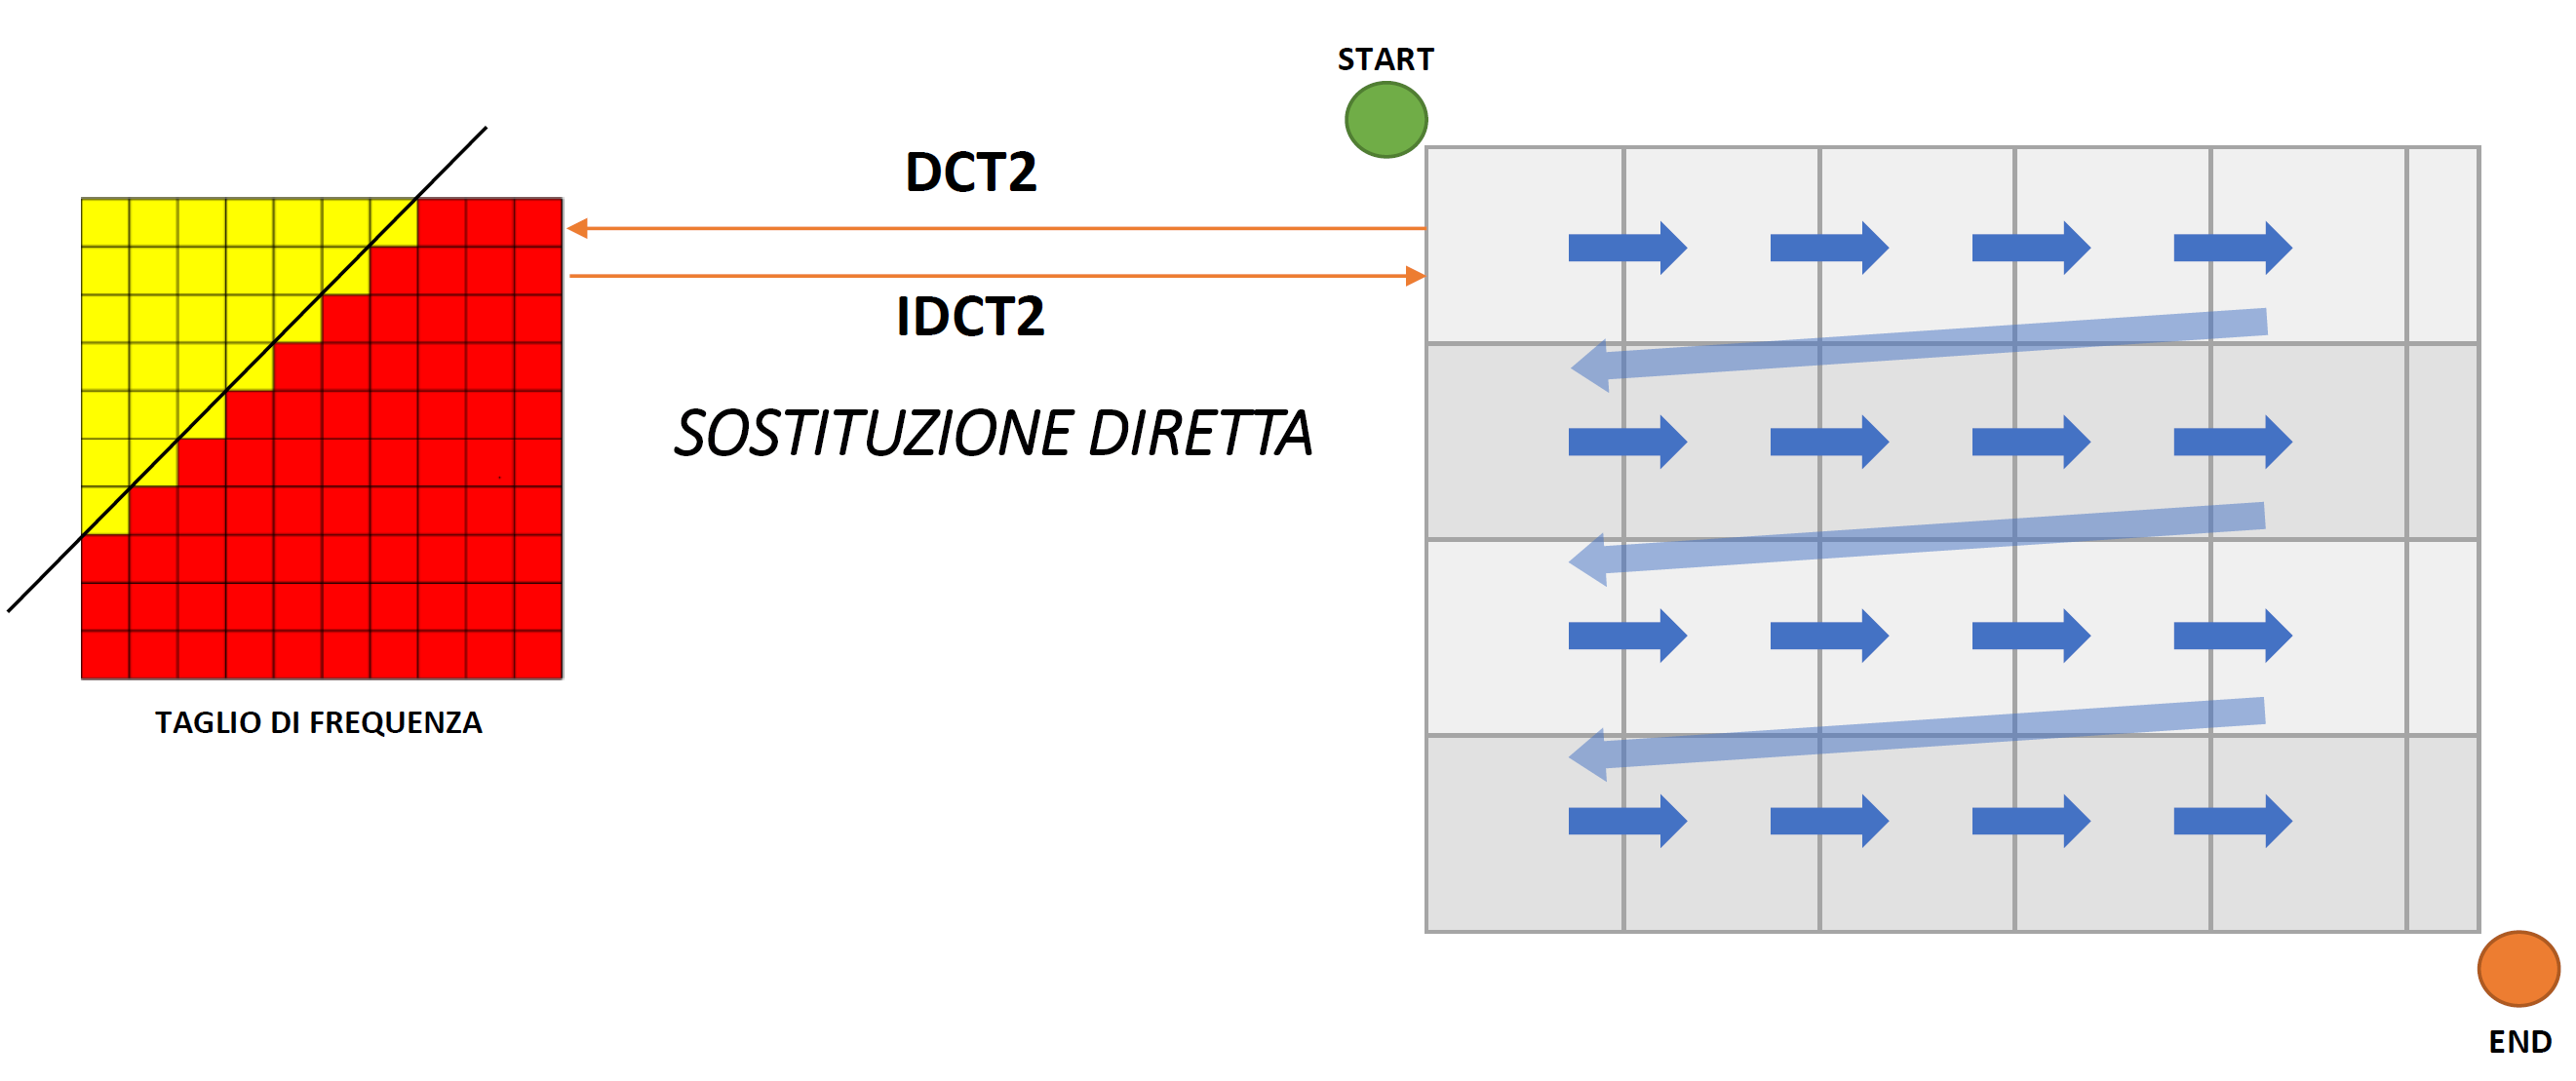
\includegraphics[width=1.2\linewidth]{flow-compression-blocks.png}}
    \caption{Compressione a blocchi}
    \label{fig:flow-compression-block}
\end{figure}

\newpage
\begin{lstlisting}[language=Python,label=code:algo-compression,caption=Implementazione in Python dell'algoritmo di compressione]
def compress_image(self):
    source = self.originalImage.pixmap.toImage()
    width, height = [source.width(), source.height()]

    # bits() -> deep copy // constBits() -> references
    values = source.constBits()
    values.setsize(height * width * 4)

    pixels = np.frombuffer(values, np.uint8).reshape((height, width, 4)).copy()
    pixels = pixels[:, :, 0].astype(np.float)

    F = self.fSlider.value()
    d = self.dSlider.value()

    height_blocks_count = int(height / F)
    width_blocks_count = int(width / F)

    for r in range(height_blocks_count):
        for c in range(width_blocks_count):
            block = dctn(pixels[r*F : (r+1)*F, c*F : (c+1)*F], norm='ortho')

            for k in range(F):
                for l in range(F):
                    if k + l >= d:
                        block[k,l] = 0

            pixels[r*F : (r+1)*F, c*F : (c+1)*F] = idctn(block, norm='ortho')

    pixels = pixels.clip(0, 255).round().astype(np.uint8)

    target = QImage(bytes(pixels), pixels.shape[1], pixels.shape[0], int(pixels.nbytes/height), QImage.Format_Grayscale8)
    self.compressedImage.setPixmap(QPixmap.fromImage(target))
\end{lstlisting}

\newpage
\section{Esempi di compressione}
\label{section:examples}
\begin{figure}[H]
    \makebox[\textwidth][c]{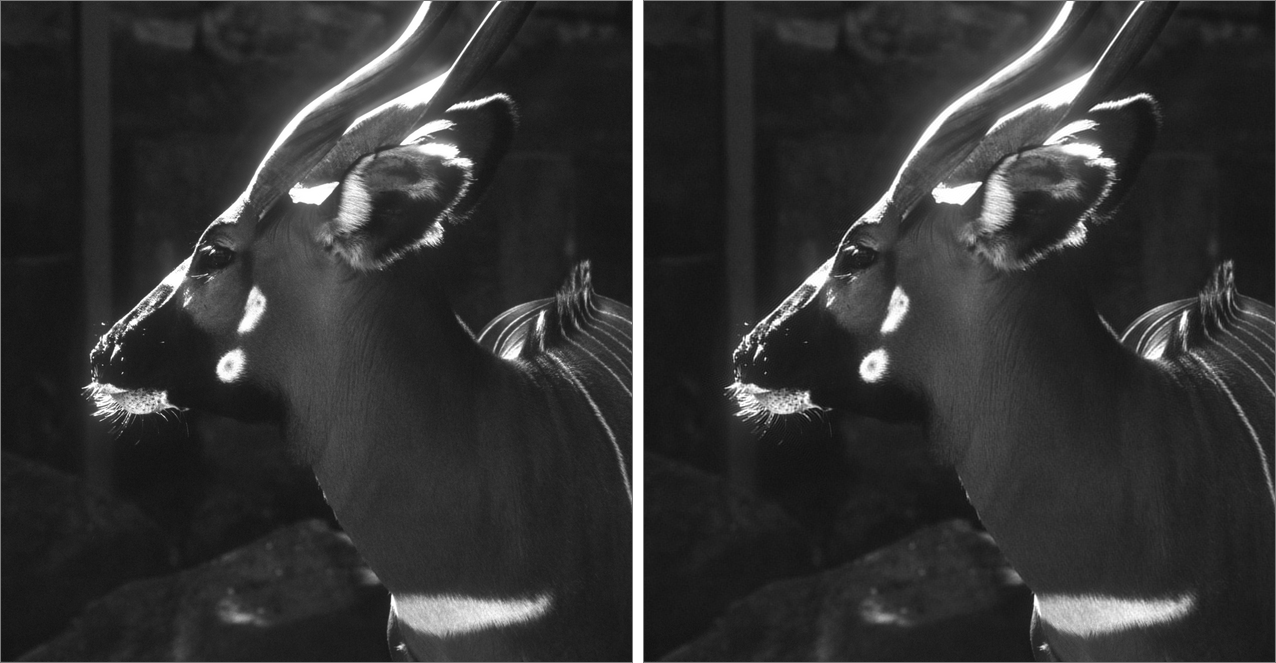
\includegraphics[width=1\linewidth]{examples/deer_1.png}}
    \caption{Parametri: $F=124$ e $d=138$}
    \label{fig:deer-1}
\end{figure}

Le \cref{fig:deer-1,fig:deer-2} mostrano la differenza nella variazione del parametro $d$, che regola il taglio di frequenza.
Pur tagliando quasi la metà delle frequenze in \cref{fig:deer-1}, questa risulta indistinguibile rispetto al file originale.

Inoltre, più viene applicata una compressione massiccia come in \cref{fig:deer-2}, più si noterà il delineamento della divisione in blocchi.

\begin{figure}[H]
    \makebox[\textwidth][c]{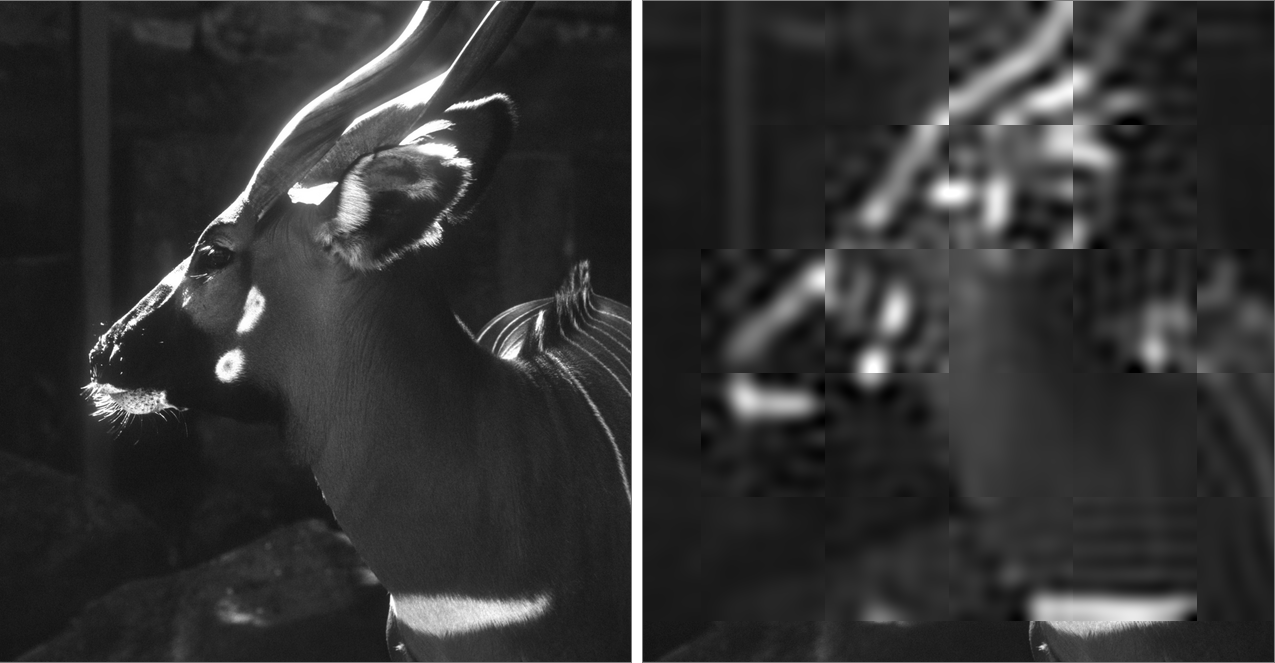
\includegraphics[width=1\linewidth]{examples/deer_2.png}}
    \caption{Parametri: $F=124$ e $d=10$}
    \label{fig:deer-2}
\end{figure}

\begin{figure}[H]
    \makebox[\textwidth][c]{
\includegraphics[width=1\linewidth]{examples/c_scale.png}}
    \caption{Parametri: $F=30$ e $d=10$}
    \label{fig:c-scale}
\end{figure}

\vfill
\noindent
Le immagini in \cref{fig:c-scale,fig:c-scale-gibbs} rappresenta, seppur in maniera lieve, il fenomeno di \textbf{Gibbs} causato dal passaggio netto dal colore nero al colore bianco (rispettivamente con valori $0$ e $255$) o viceversa, manifestandosi come un aloni che seguono i contorni della C e del cervo.

\vfill
\begin{figure}[H]
    \makebox[\textwidth][c]{
\includegraphics[width=1\linewidth]{examples/c_scale_gibbs.png}}
    \caption{Fenomeno di Gibbs / Parametri: $F=100$ e $d=98$}
    \label{fig:c-scale-gibbs}
\end{figure}

\newpage
\noindent
Dall'immagine \cref{fig:deer-gibbs} si può osservare un comportamento piuttosto interessante: il fenomeno di Gibbs si propaga esclusivamente all'interno del blocco nel quale si verifica.

Proprio per questo motivo, la compressione JPG classica pur operando in modalità differente, utilizza blocchi di dimensione $F$ molto piccoli (solitamente $8\times 8$).

\begin{figure}[H]
    \makebox[\textwidth][c]{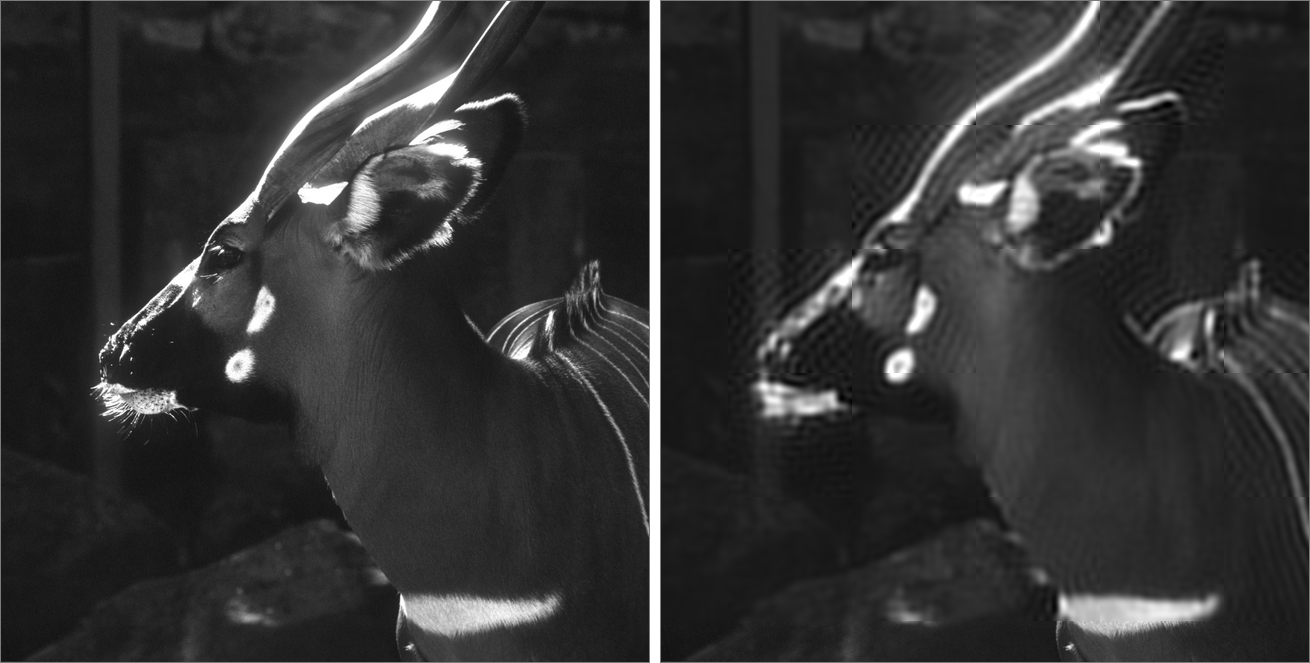
\includegraphics[width=1\linewidth]{examples/deer_2_gibbs.png}}
    \caption{Fenomeno di Gibbs / Parametri: $F=124$ e $d=28$}
    \label{fig:deer-gibbs}
\end{figure}

% deep_1 = 124 e 138
% deep_2 = 124 e 10
% c_scale = 30 e 10
% c = 30 e 10

\newpage
\section{Osservazioni}
\begin{enumerate}
    \item Le immagini richiedono di lavorare con i 4 tipi di canale: RGBA che in combinazione definiscono il colore.
\end{enumerate}
La traccia richiede di lavorare con immagini in toni di grigio, dalle analisi fatte(come in figura in alto a destra) si nota che il valore di \textit{un qualunque grigio} è uguale per tutti i canali.\newline
Di conseguenza si è deciso di lavorare con un solo canale (in questo caso il primo, ovvero Red).
\begin{enumerate}
    \item Quindi l’immagine viene divisa in blocchi f di pixels di dimensione F x F, partendo dal primo blocco in alto a sinistra;
    \item Per ogni blocco si effettuano le seguenti attività:
    \begin{enumerate}[label=\Alph*]
        \item Si applica la dctn (DCT2 della libreria): c = DCT2(f);
        \item Vengono eliminate le frequenze ckl con k+l >= d;
        \item Si applica idctn sulla matrice c: ff = IDCT2(f)
    \end{enumerate}
\end{enumerate}


\end{document}